\chapter{Methodology} \label{ML}

\section{Introduction :}\label{contextofimp}
In this chapter we will review each of Classical approaches, Autoregressive model ARIMA, VAR and Deep learning models, then discuss each model  limitation's and Pros & Cons.
the data used is a traffic data set with a whole lot of missing data, which gives us a dirty ground to test our models on and benchmark them against each others.\\We will also review some of the models that failed to fulfill our project's needs, Finally we will discuss the possibility of using Transfer Learning to impute missing data in the field in real time.



\section{Data used}
the  data used in this project, is a real world traffic data, it was collected from  monitoring stations located between Nancy and  Metz  A31  road ''La Direction Interdépartementale des Routes Est (DIR Est) '', the idea of the project is to study  how  a set of speed limits displays that change in time dependent on a lot of factors, would actually reduce the traffic congestion.
and for that they took measures of Speed and Flow rate, of course there other Spatial features like the section of sensor (refered to as station), there are also 2 sens and some times 3 sens in a road, and other features that allocate spatially where sensors are.
but one thing let their Data scientist, struggle to have a conclusion was Missing Data values.


\begin{figure}[H]
\centering
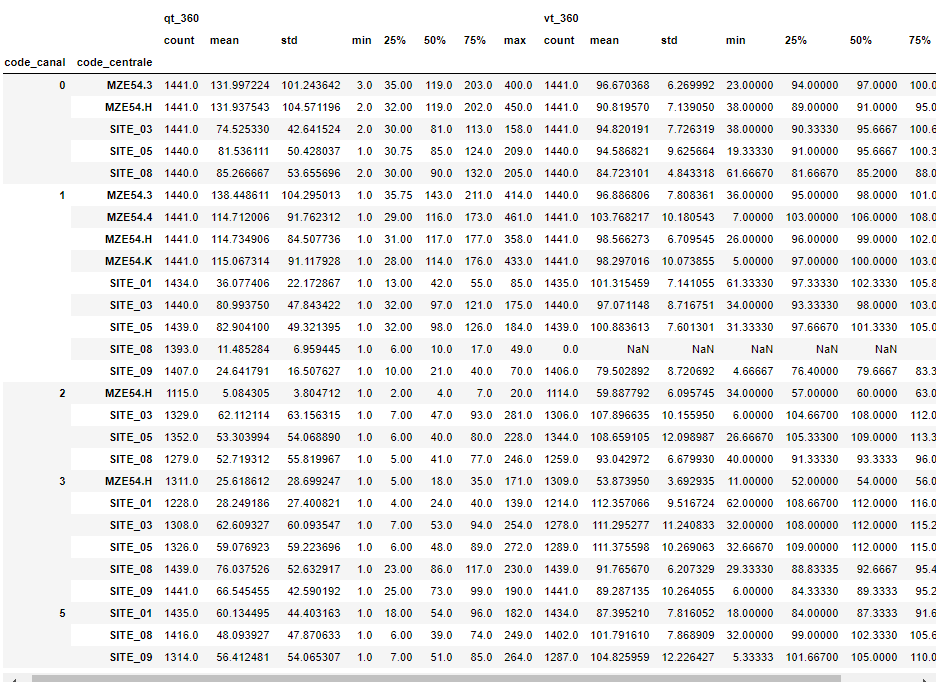
\includegraphics[scale=.53]{img/grouped_data_descriptives.png} 
\caption{traffic Dataset descriptive statistics}
\label{fig:score}
\end{figure}


\section{classical methods :}

the distribution of missing data is not following any pattern, which favor the hypothesis of being Missing at random, which is the case of 90\% in real world data.

%
\begin{figure}[H]
\centering
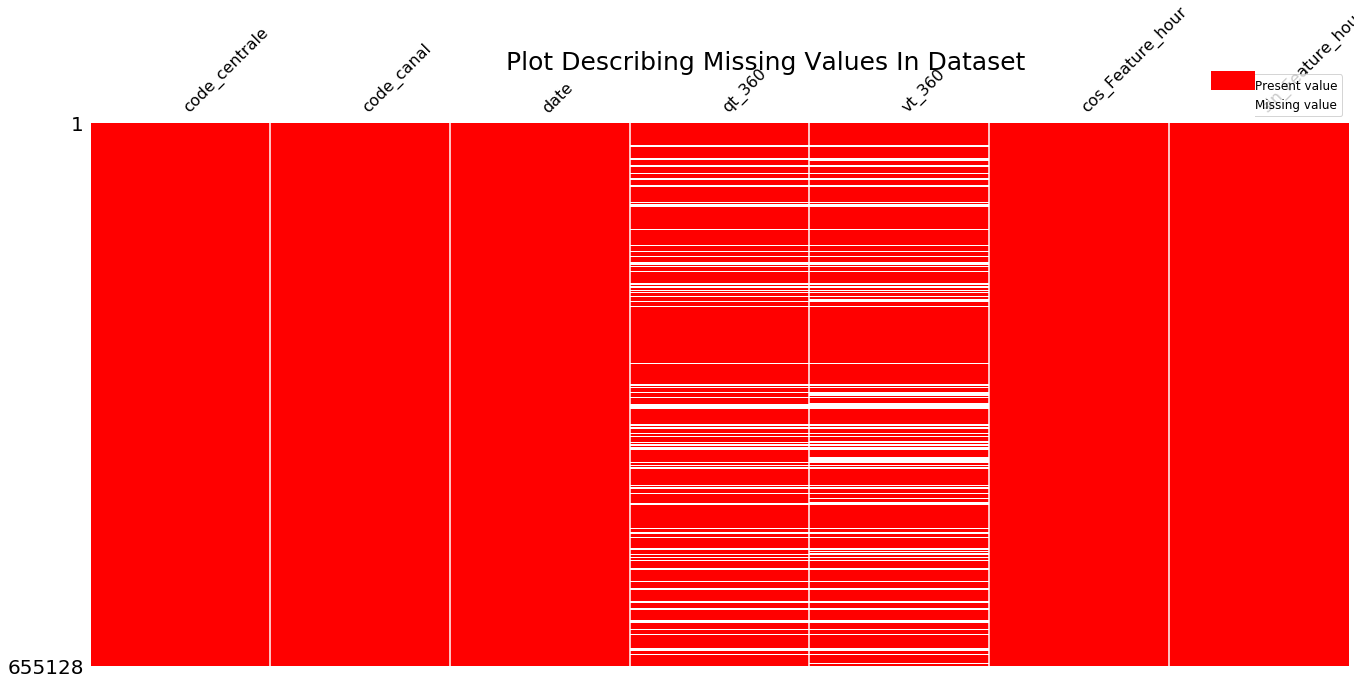
\includegraphics[width=.9\textwidth]{img/missing_values_distributation.png} 
\caption{Missing data distribution of all features in Dataset}
\label{fig:presteps}
\end{figure}
%

the naive solution is to impute (fill) missing values using mean values of each feature. which seems reasonable estimate except that this is not safe to use even if your missing observation are completely at random. However, clearly this is not the case we are dealing with, the mean  method may lead to inconsistent bias. 

The figure below shows the imputation  using Mean and Standard Deviation,  here we have a gap of 3 days, No additional information was added, the mean only make  the size of time serie bigger, this leads to an underestimate of the errors [\ref{}].
%
\begin{figure}[H]
\centering
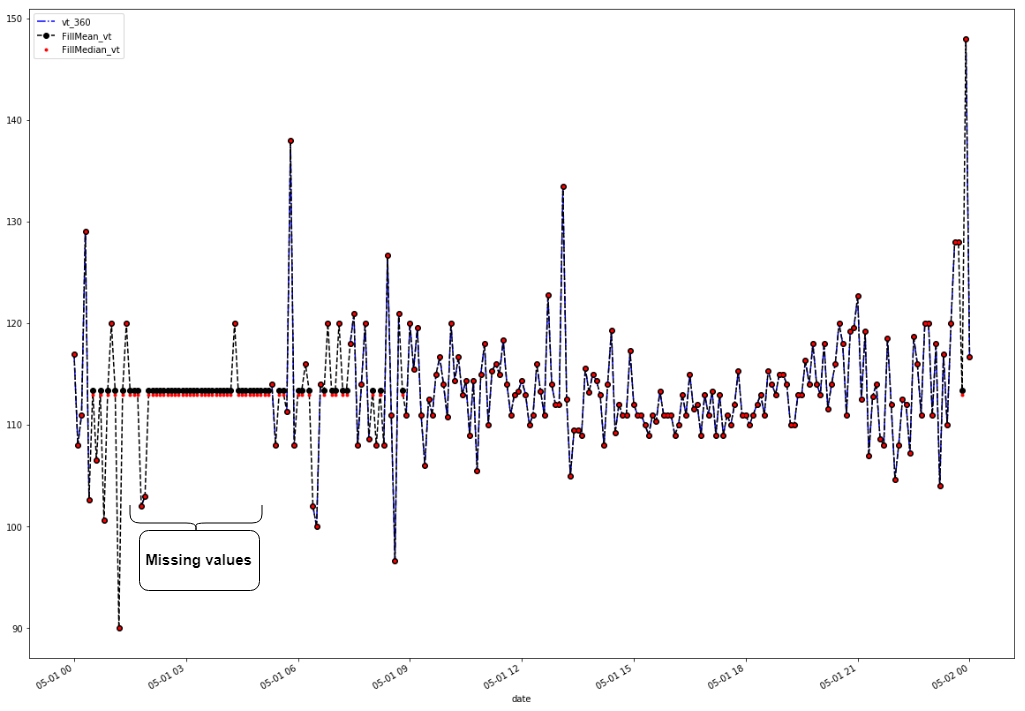
\includegraphics[scale=.4]{img/mean_median.png} 
\caption{Mean and standard Deviation imputation}
\label{fig:presteps}
\end{figure}
%
on the other hand one may try only to interpolate using linear interpolation or even add more polynomial degrees, and quantify the error made by different interpolation techniques.

\begin{figure}[H]
\centering
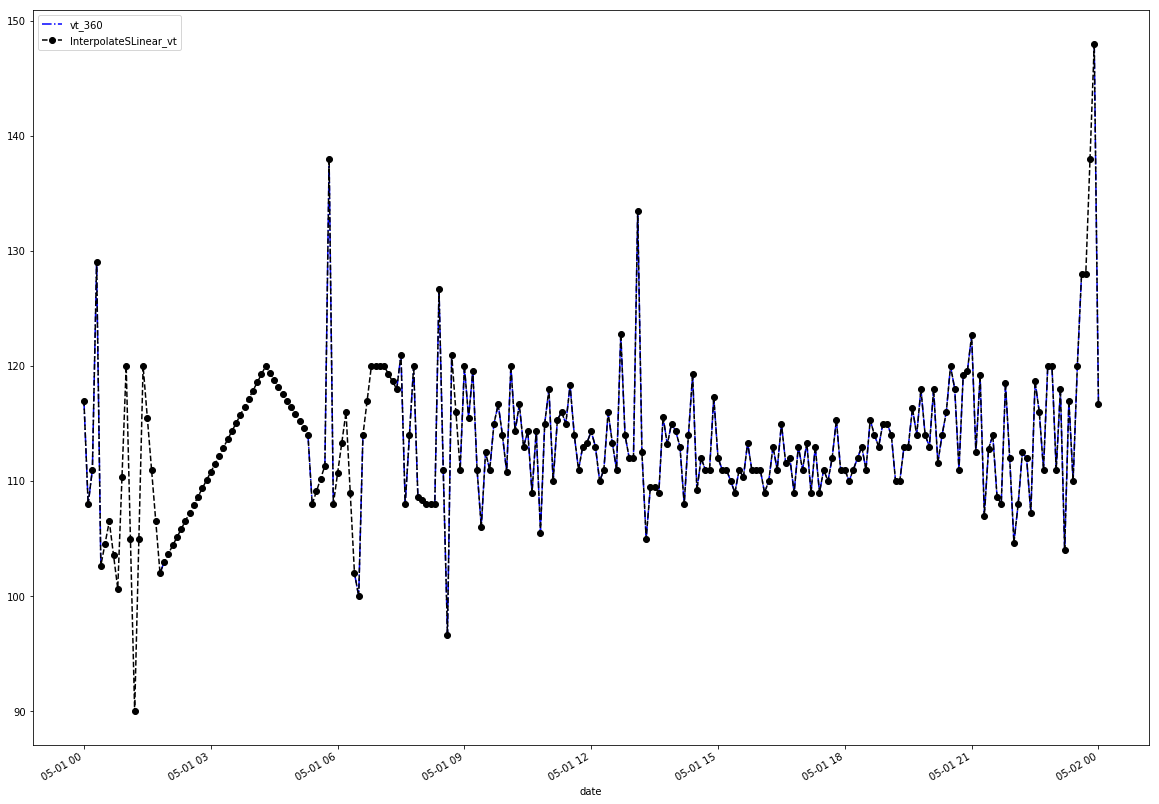
\includegraphics[scale=.33]{img/linear.png} 
\caption{Imputation using Linear Interpolation }
\label{fig:presteps}
\end{figure}


%
% \begin{figure}[H]
% \centering
% 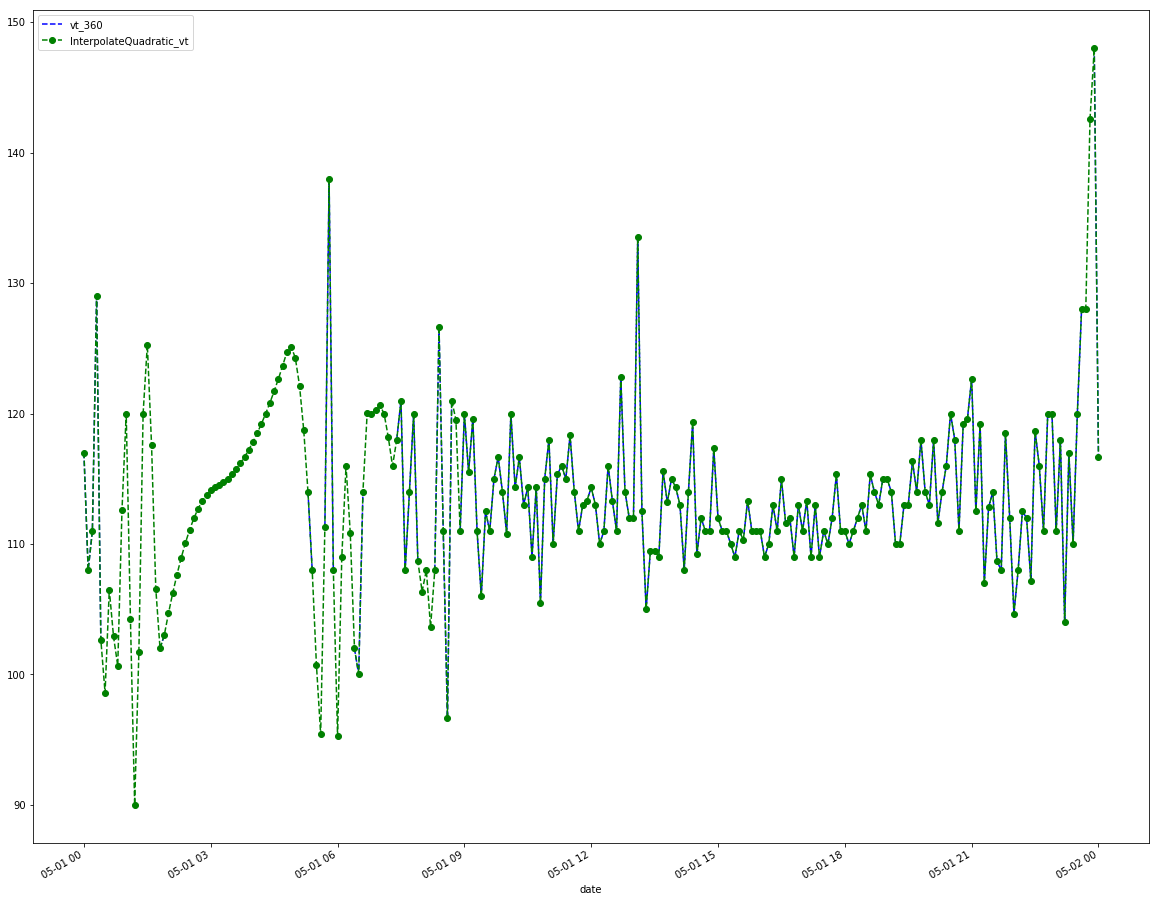
\includegraphics[width=.75\textwidth]{img/quadratic.png} 
% \caption{Imputation using Quadratic Interpolation}
% \label{fig:presteps}
% \end{figure}

% %
% \begin{figure}[H]
% \centering
% 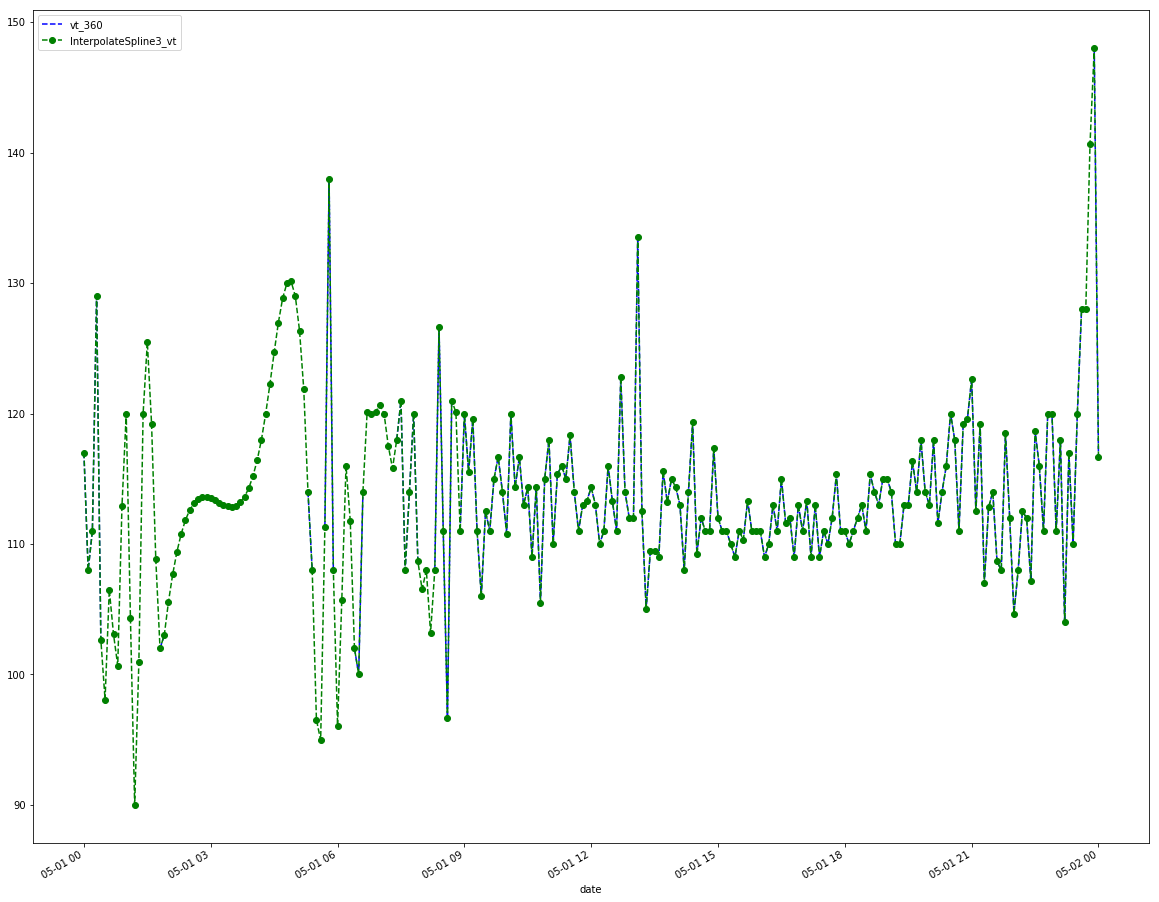
\includegraphics[width=.75\textwidth]{img/spline.png} 
% \caption{Spline interpolation for imputation}
% \label{fig:presteps}
% \end{figure}
%%

\begin{figure}[h]
\centering
\begin{minipage}{.49\linewidth}
    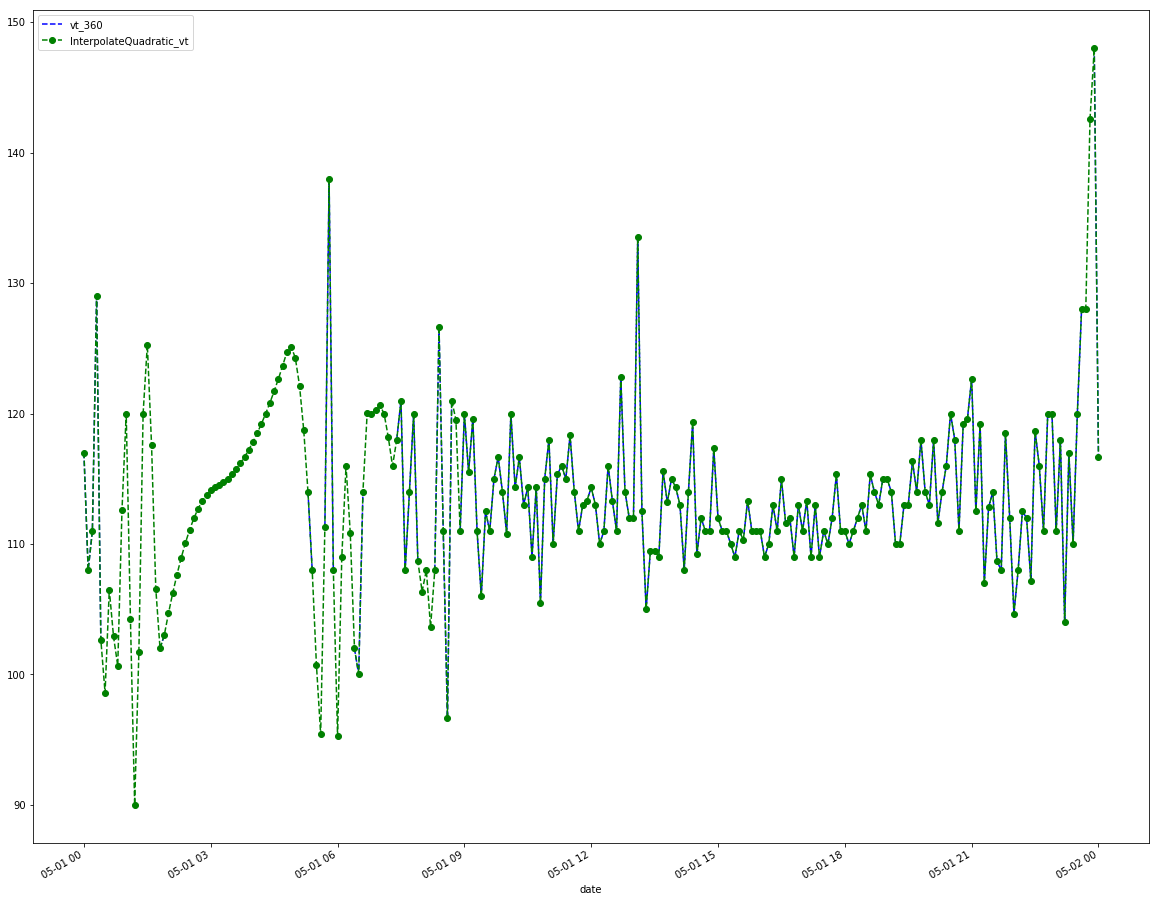
\includegraphics[width=.9\textwidth]{img/quadratic.png}    
    \caption{Quadratic Interpolation}
    \label{img1}
\end{minipage}
\hfill
\begin{minipage}{.49\linewidth}
    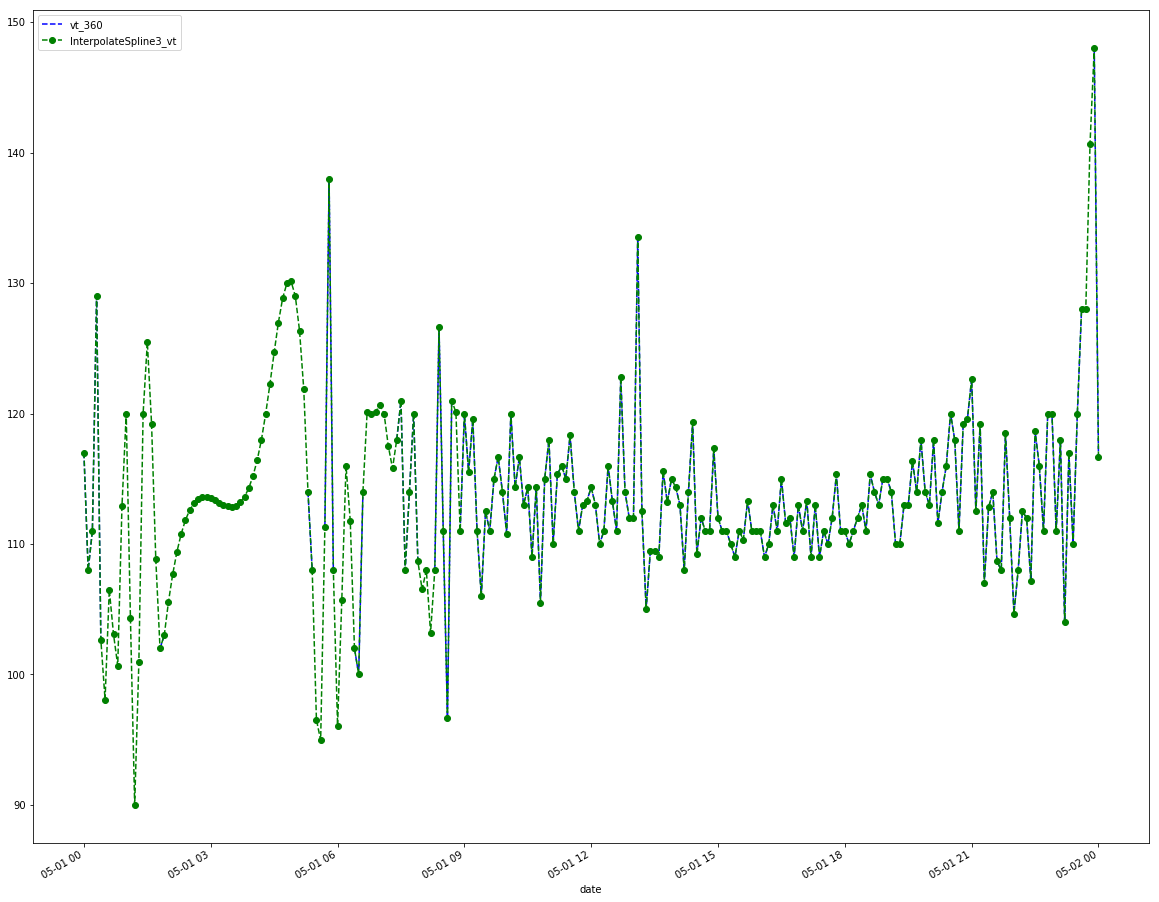
\includegraphics[width=.9\textwidth]{img/spline.png} 
    \caption{Spline interpolation for imputation}
    \label{img2}
\end{minipage}
\end{figure}


Scoring the results and see which is better, we can see from figure below [\ref{fig:score}], that both linear interpolation and interpolation Time is giving the minimum error compared to other methods.

\begin{wrapfigure}{!l}{0.35\textwidth}
\centering
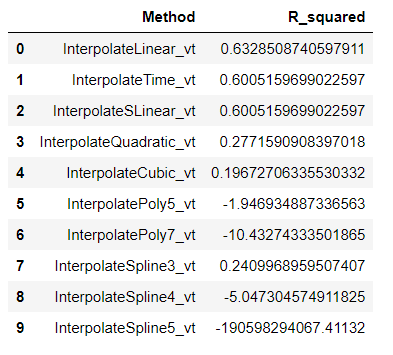
\includegraphics[width=.4\textwidth]{img/results_R.png} 
\caption{Missing data distribution of all features in Dataset}
\label{fig:score}
\end{wrapfigure}
we can see clearly how inefficient these methods are and can introduce bias data to work with later or train on.thus, these methods cannot be employed, as they are not  based on inter-variable correlations, neither they take the time dimension into account as a major feature in order to estimate missing values. For instance the interpolation methods tries to fit a “smooth curve” fitting the observed data and this way we approximate the missing values but with a really poor hypothesis that will need a lot of constraints to be true. Also it discards any relationships between the variables over time. Other methods that are usually used for times series predictions ( the autoregressive methods like ARIMA) can hold the answer for our problem.


\section{ ARIMA (Autoregressive Integrated Moving Average):}
as we already mention in state of the art ARIMA is a very famous method for forcasting in finance and Time Series Data,  
Box and Jenkins proposed a set of guidelines that can be followed when
selecting ARIMA models. This systematic procedure to designing ARIMA
models has made them highly popular (Hibon and Makridakis
\protect\hyperlink{ref-spyros1997}{1997}).  It consists of a four-stage iterative process in which:

\begin{enumerate}
    \item  the process is either transformed or
differenced to de-trend\ref{fig:detrend} and stabilise the variance of the data.
 

\begin{figure}[H]
\centering
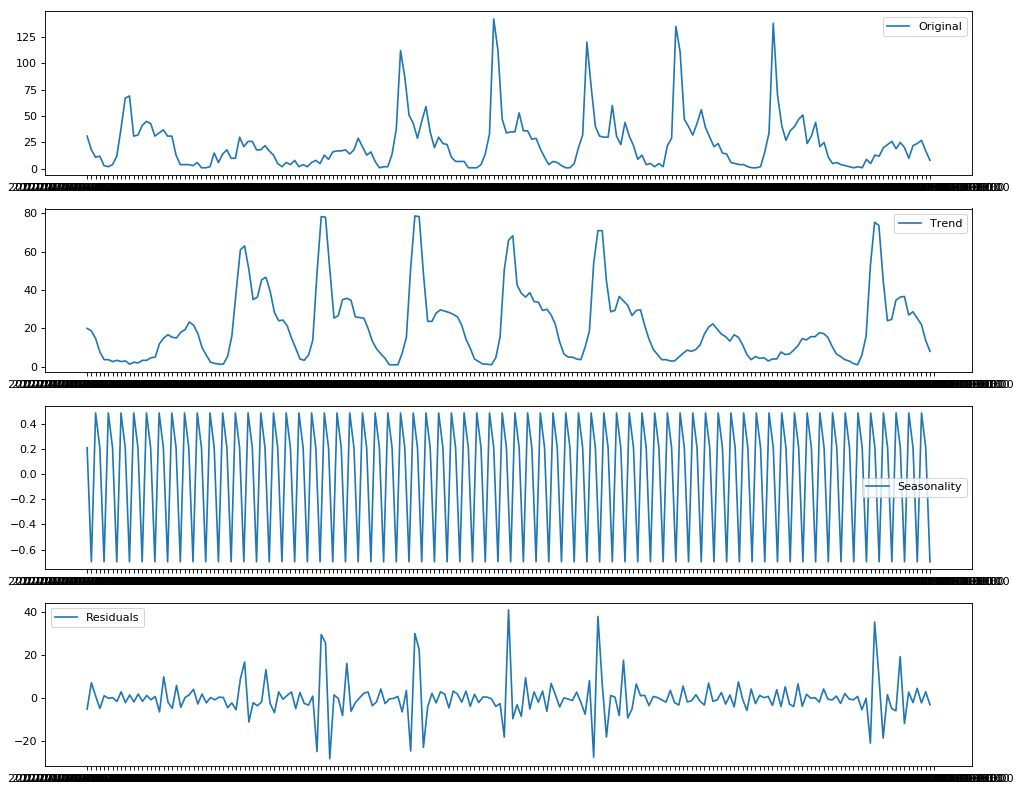
\includegraphics[scale=.4]{img/detreding.png} 
\caption{Remove trend and seasonality with decomposition }
\label{fig:detrend}
\end{figure}

\item the autocorrelation and partial autocorrelation plots are used to determine the order of p and q,
\item the parameters of the model are estimated,
\item a diagnostic check is performed to ensure that the residuals are a white noise process. If the residuals are not white noise steps 2-4 are repeated until a satisfactory model is identified. On the contrary, if the diagnostic check shows that the residuals are random then the developed model is the final model used for forecasting.
\end{enumerate}

It is important to keep in mind that regression techniques works on  observations that are independent of each other, we know that in time series all variables are time dependent, unless the time serie is Stationary we can not use any regression model.

To do so, we use  Dickey-Fuller test \ref{dickeyfuller}, a statistical test with the null hypothesis that the time series is non-stationary. If the test results in the test statistic significantly less than the critical values, we can reject the null hypothesis in favor of time series stationarity.

as we may see in the figure below \ref{fig:duckeytest} our time serie is stationary :

\begin{figure}[H]
\centering
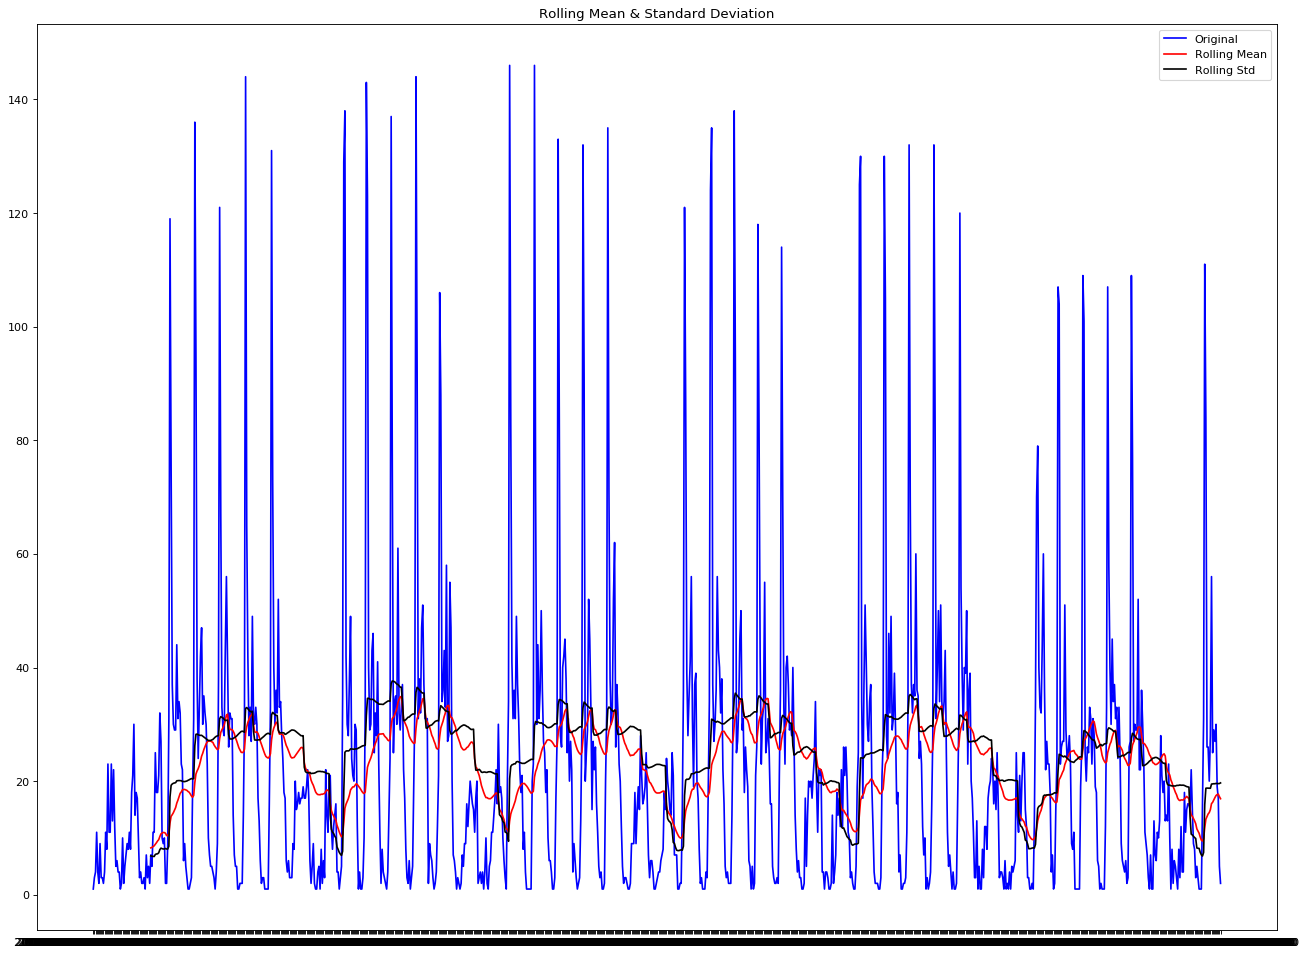
\includegraphics[scale=.35]{img/duckeyTest.png} 
\caption{imputation using Linear Interpolation }
\label{fig:duckeytest}
\end{figure}

Results of Dickey-Fuller Test:
\begin{wraptable}{!}{70mm}

\begin{tabular}{lllll}
\cline{1-2}
\multicolumn{1}{|l|}{\begin{tabular}[c]{@{}l@{}}Test Statistic                  \\ p-value                          \\ \#Lags Used                      \\ Number of Observations Used   \\ Critical Value (1\%)             \\ Critical Value (5\%)             \\ Critical Value (10\%)\end{tabular}} & \multicolumn{1}{l|}{\begin{tabular}[c]{@{}l@{}}-3.634985\\ 0.005126\\ 22.000000\\ 977.000000\\ -3.437061\\ -2.864503\\ -2.568348\end{tabular}} &  &  &  \\ \cline{1-2}
\end{tabular}
  \caption{Dickey-Fuller Test}

\end{wraptable}


The order of differencing is determined by using the KPSS test (Ruppert and Matteson\cite{RaM}). The KPSS test checks the null hypothesis of stationarity and sets d to zero if the null hypothesis is accepted, otherwise it iteratively increases d by 1 and tests the null hypothesis until it is accepted (Ruppert and Matteson \cite{RaM}). Once the order of
differencing has been determined, the order of p and q are chosen based on Akaike's Information Criterion (AIC) or the Bayesian Information Criterion (BIC).


Due to the large number of forecasts made, it is useful to have an
automatic procedure which is able to select the appropriate ARIMA model to fit the data. The \textbf{auto Arima} function in python, available also in R  is able to automatically choose the order of the parameters p, q and d.


\begin{figure}[H]
\centering
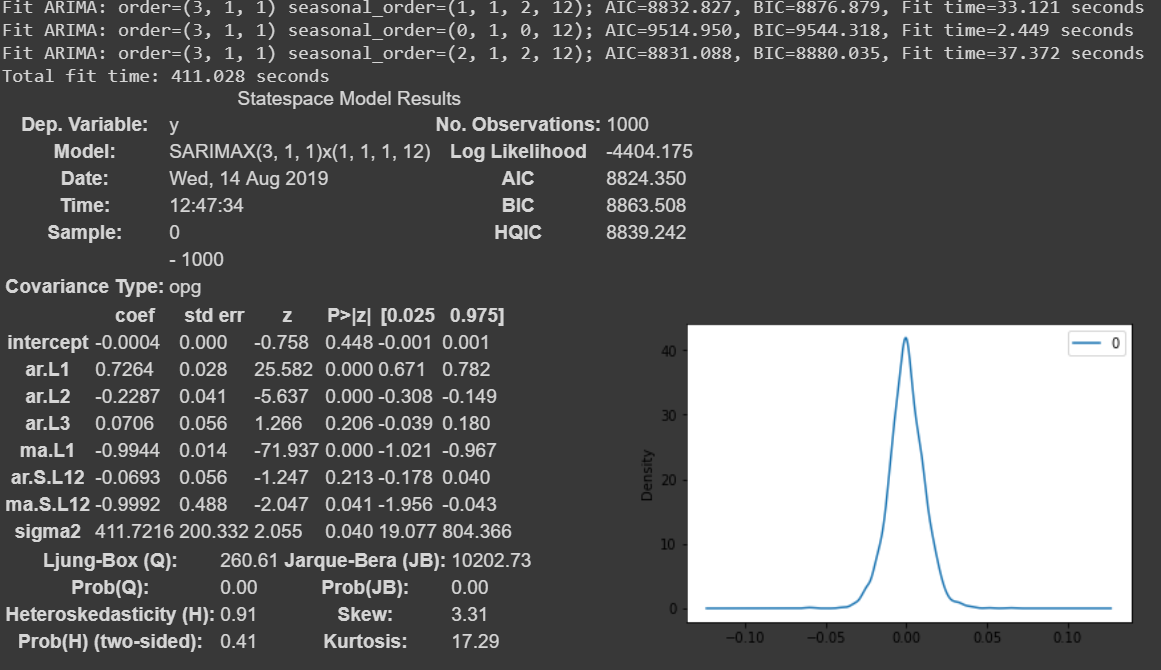
\includegraphics[scale=.6]{img/arima_degrees.PNG} 
\caption{Missing data distribution of all features in Dataset}
\label{fig:arima_degree}
\end{figure}

In order to validate the ARIMA model appropriateness is by performing residual analysis.

Print the results of the ARIMA model and plot the residuals as show in figure \ref{fig:arima_degree}. A density plot of the residual error values indicates a normal distribution centered around zero mean. Also, the residuals do not violate the assumptions of constant location and scale with most values in the range (-1,1).



in the next figures we can see the inference of  the best selected model with order=(3, 1, 1) and seasonal order=(2, 1, 2, 12). which scored an RMSE of 0.8 on the training data as in fig\ref{fig:trainig_arima}, we can forecast future event by just fitting the Arima model on the last  known data and have a forecasting as shown in figure \ref{fig:forcasting}.  


\begin{figure}[H]
\centering
\begin{minipage}{.49\linewidth}
    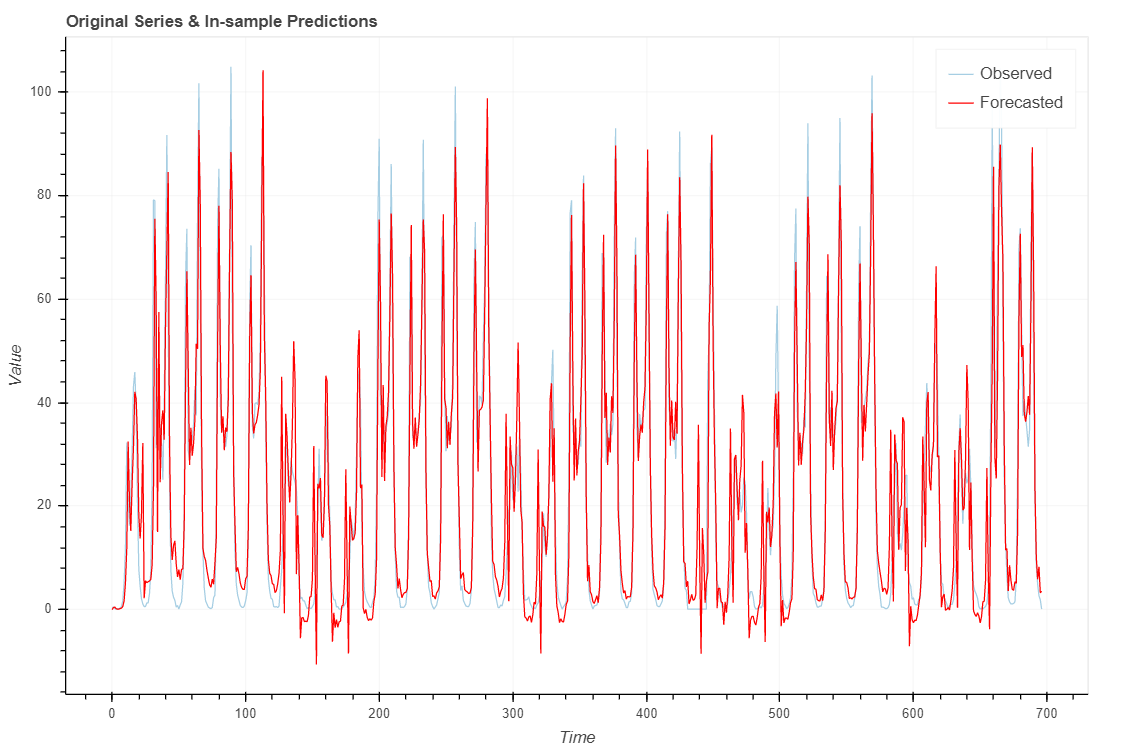
\includegraphics[width=.9\textwidth]{img/arima_training.png}    
    \caption{Arima prediction on training data}
    \label{fig:trainig_arima}
\end{minipage}
\hfill
\begin{minipage}{.49\linewidth}
    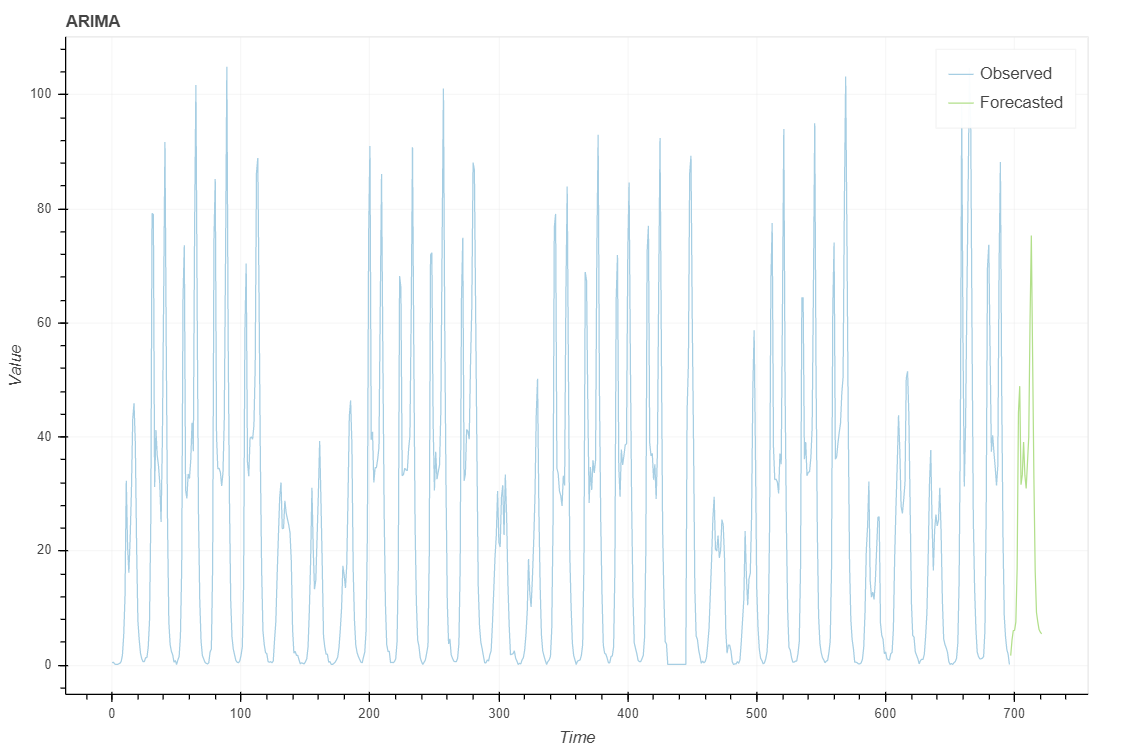
\includegraphics[width=.9\textwidth]{img/arima_forcasting.png} 
    \caption{Arima Forecasting}
    \label{fig:forcasting}
\end{minipage}
\end{figure}

%
\begin{verbatim}
MAE : Train Score: 3.48 , Test Score: 2.2
RMSE : Train Score: 3.53 , Test Score: 3.62
\end{verbatim}



now the idea as mentioned before is to go back to each gap and impute as if we want to infer and forecast the gap, The figure shown below shows the results obtained by imputing (filling), missing data by arima forecast.

\begin{figure}[H]
\centering
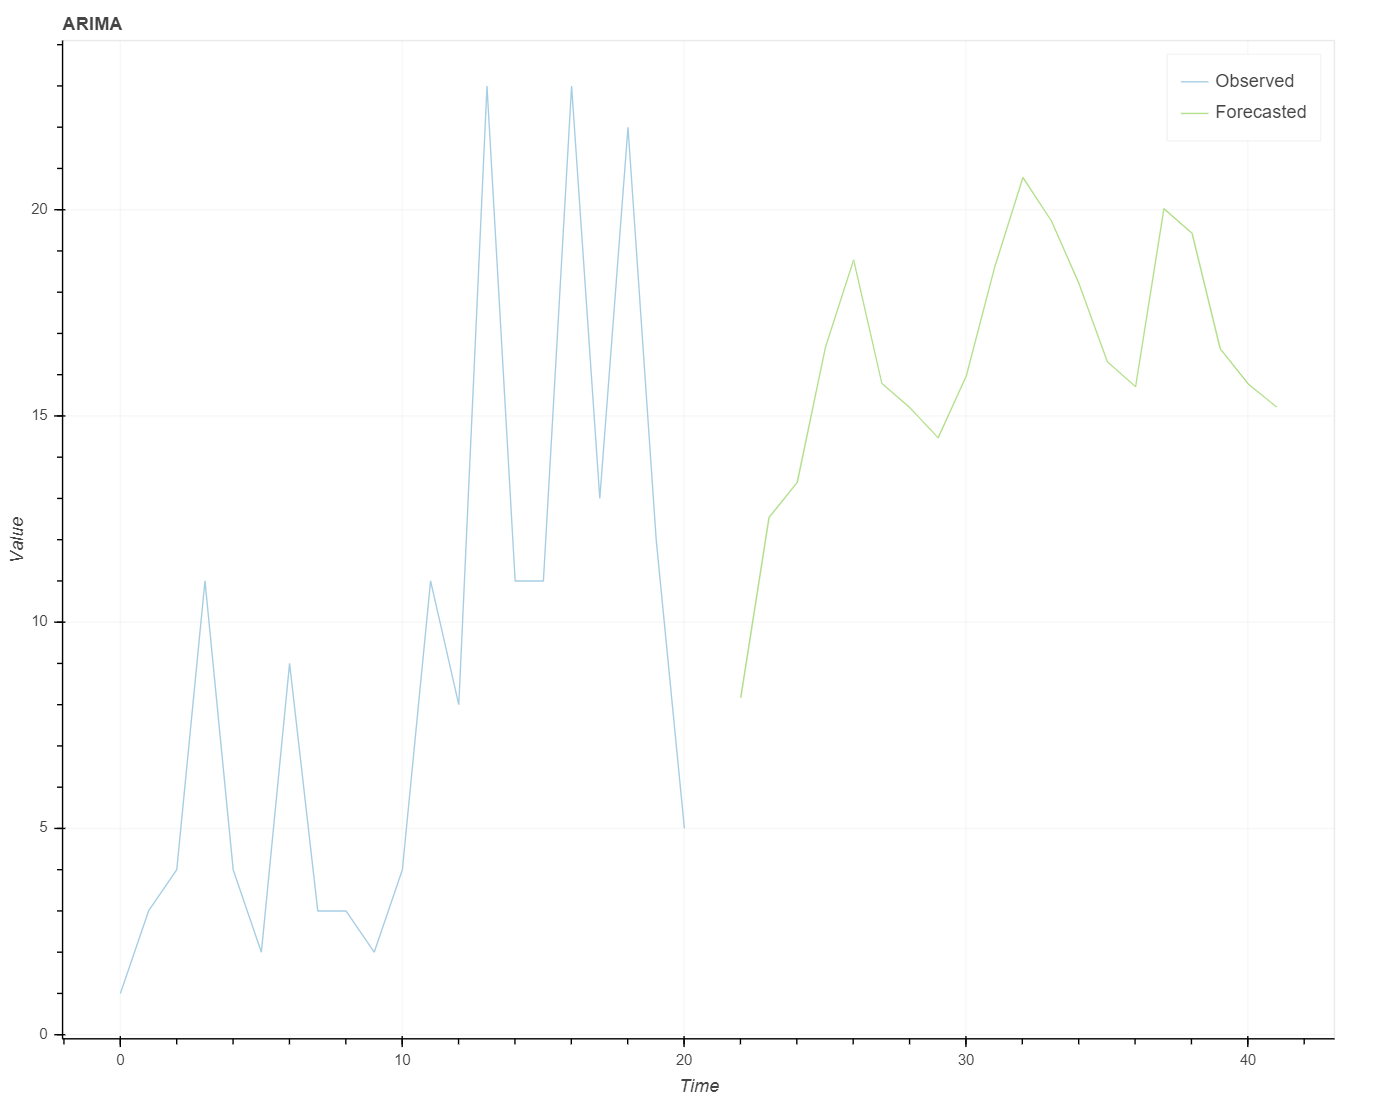
\includegraphics[scale=.2]{img/arima_imputation.png} 
\caption{Arima imputation}
\label{fig:arima_degree}
\end{figure}
often  in practice we use a kalman smoother to interpolate. 

Arima is good pratice for time series data and can give good result especially if you have small set of data, except that it eliminates the non-stationary parts in time series data and fit a parameterized stationary model, Also one of the biggest constraints why we can not proceed with ARIMA  is that we usually have multiple variables we need to use in order to impute  a damaged sensor, we need a model that can uses other's features to impute the missing data. 

As we have seen earlier the two models that can have a good modeling for time series and also  take into consideration all other features, are  Vector Auto-regressive (VAR) or Recurrent Neural Networks (RNN).

in  our Benchmarking, the VAR failed badly to fit even the Training Data, this is due to large amount of features. 

\begin{figure}[H]
\centering
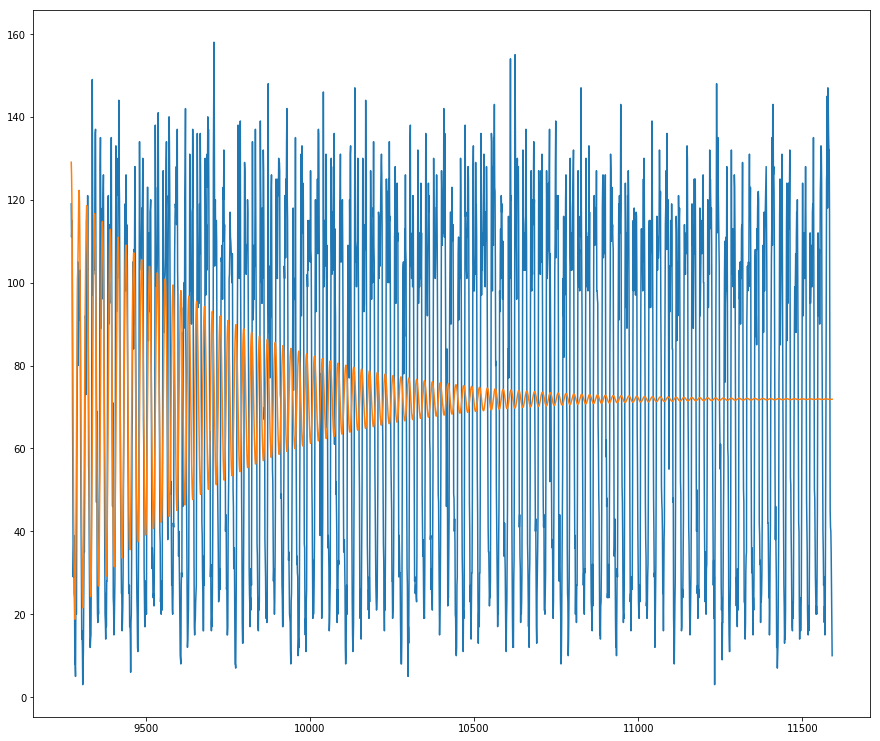
\includegraphics[width=.5\textwidth]{img/VAR.png} 
\caption{Vector Autoregressive VAR}
\label{fig:arima_degree}
\end{figure}

that left us with Deep learning approaches, Time series are sequential data whereas RNN is the state of the art to deal with sequential data.
\section{Deep learning :}
\subsection{Building the RNN}
The RNN used was built on top of Keras API\cite{keras2015} with tensorflow  back-end. we used a variant of RNN called LSTM  that can even learn from larger dependencies, the coming list represents the specifications of the architecture used in this project:
\begin{itemize}
\item we used a the Many to one RNN architecture  uses a single output feed forward node as shown in figure \ref{fig:manyto_one}.

\begin{figure}[H]
\centering
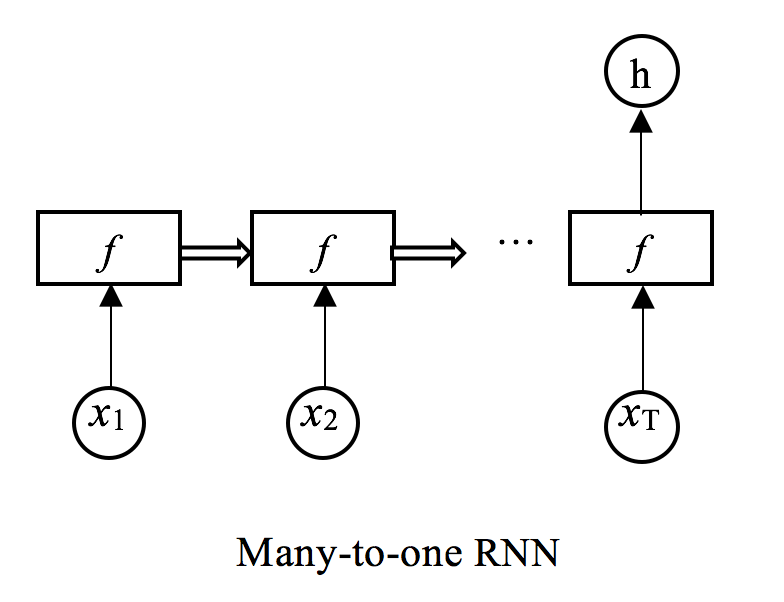
\includegraphics[scale=.3]{img/many_to_one.png} 
\caption{input as many time steps in the sequence, but the model produces only one output to predict the t+1 .}
\label{fig:manyto_one}
\end{figure}

    \item This architecture uses  $sigmoid$  as activation function for the output layers\ref{fig:lstmcell}.
    \item the activation function for the recurrent node was $tanh$ \ref{fig:lstmcell} .
\end{itemize}

\begin{figure}[H]
\centering
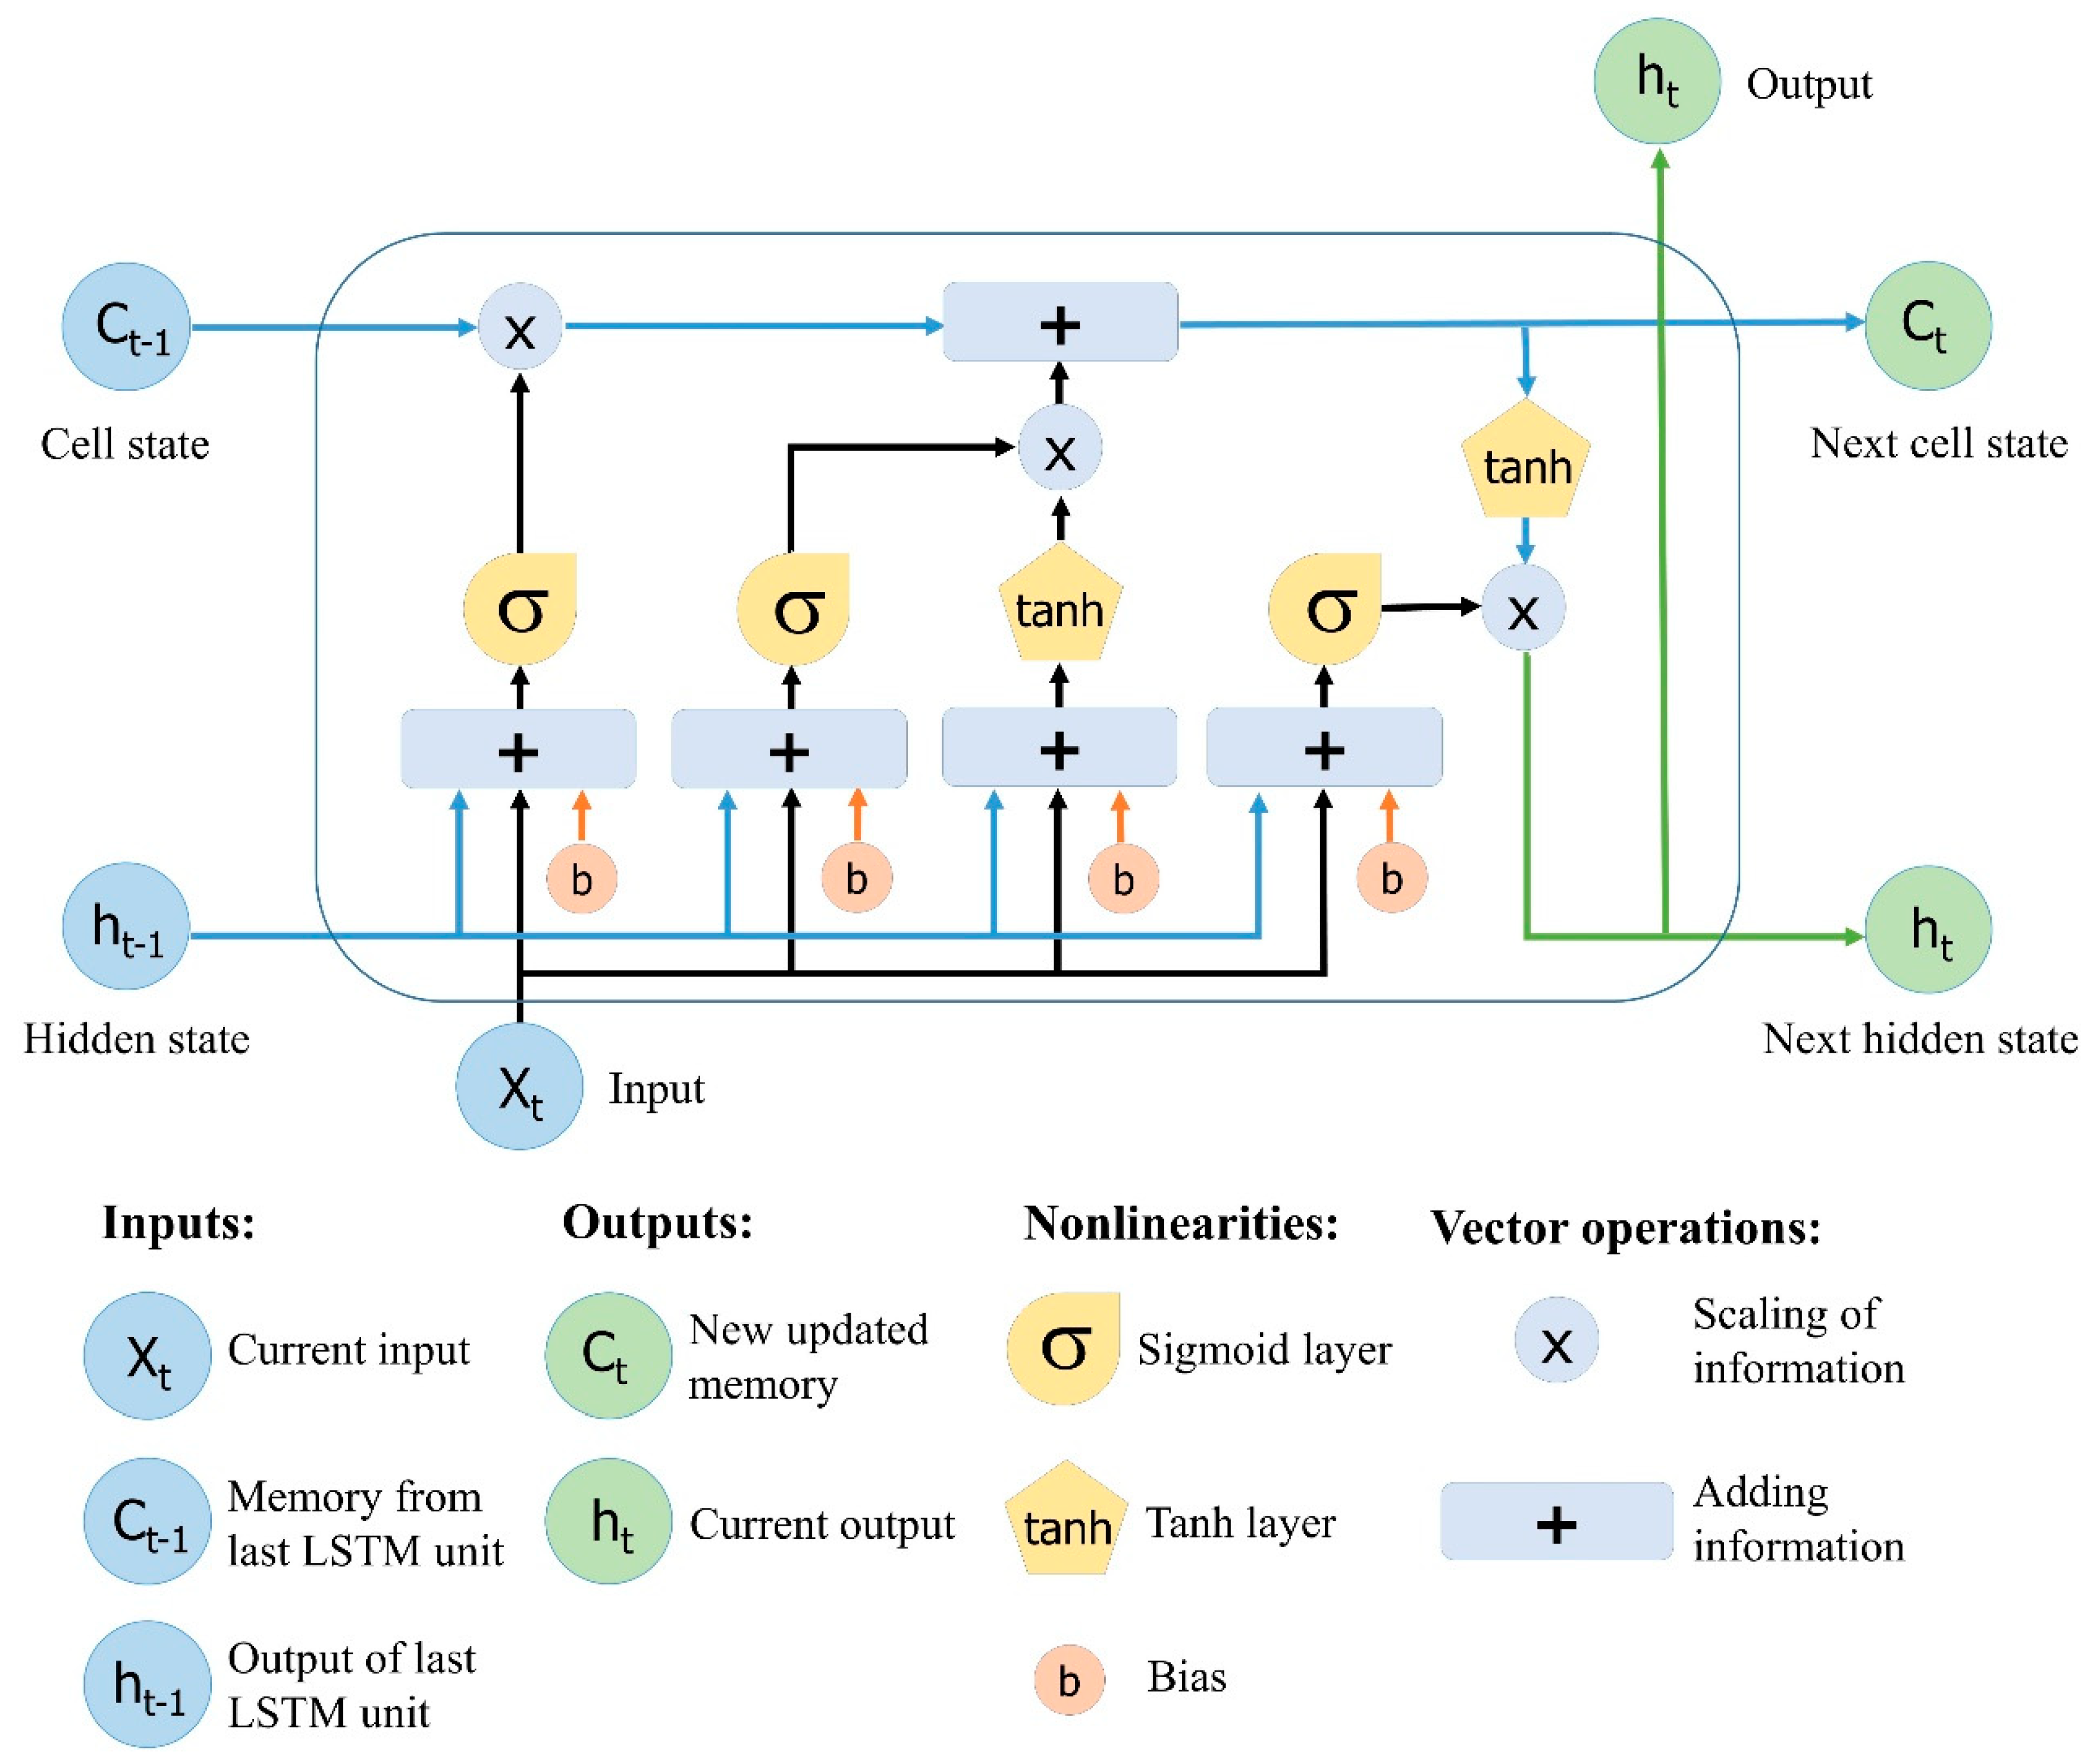
\includegraphics[scale=.55]{img/The_LSTM_cell.png} 
\caption{The Long Short-Term Memory (LSTM) cell can process data sequentially and keep its hidden state through time. image is taken from  \cite{}}
\label{fig:lstmcell}
\end{figure}

basic LSTM model consisted of two layers with  150 neurons in each layer, 0.2 dropout for regularization that drops nodes which prevent our model from overfitting, data is given in a batch size of 50 and 50 epochs.



\subsection{Pre-processing \&  Data preparation}
the training data was pre processed first to identify  outliers, a value was considered an outliers if it is 3 times greater than feature mean. we also add additional information in the form of  binary filter that indicates where missing that is, if a value is missing was marked 1.\\ 
Another way to mark missing data is the time delay between two consecutive non missing values.
Date is a a valuable data $Days\ ,Hours\ and\ Months$ can not be passed directly in their original form, that will be awfully misleading for our network since our network can not handle on its own the modulo operation. to prevent this problem  from happening we turn data into a cyclic data by decomposing it into pair of cosine and sine.
All these meta data will give additional information to train on.

As we are going train a large network, we would want to scale our data first between [0-1] in order to converge. and for that we transformed data between values 0 and 1 \cite{Chatterjee2017} using the \textbf{MinMaxScaler} function \ref{eq:MaxMin}.
%
\begin{equation}
\label{eq:MaxMin}
x_{scaled} = \frac{x_{i} - x_{min}}{x_{max} - x_{min}}
\end{equation}
%

\subsection{Output data preparation}
The LSTM was trained to predict 1 hour ahead, to do so we shift back our data to the last $look\ back$ sequences or time steps, it is important to remember that in order to predict sequence at time t+1 we " $look\ back$ "  at the last \in$ \left\{t,t-1,t-2,t-3...t-n\right\}$ with 'n = $look\ back$'  which is parameter to tune later in order to find the best value for it.


\subsection{Tensor Preparation for RNN input data}
Data sets is passed to the LSTM in a 3D tensor, where the first parameter is a batch dimension $n$, represents the number of observation we can process in parallel, the second parameter refers to the number of time steps or look back parameter that decide how many time steps we are going back to see in past in order to predict one sequence ahead in future, the third parameter is the number of features of our data set. for more illustration the figure below shows how data is feed into the LSTM network \ref{fig:tensor-tables} 
  
%
\begin{figure}[H]
\centering
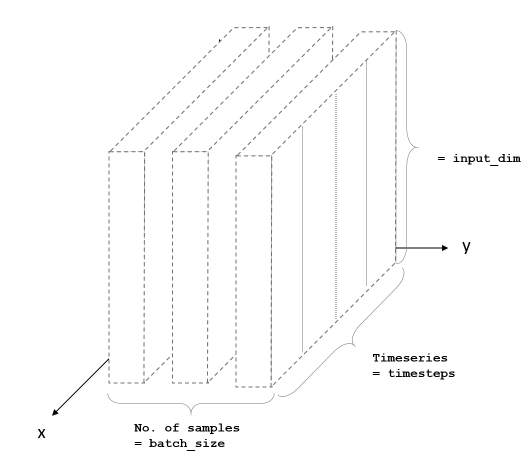
\includegraphics[scale=.45]{img/tensor.PNG}  
\caption{Process of converting data input columns into a Tensor for training the RNN \cite{tensor}.}
\label{fig:tensor-tables}
\end{figure}
%

\subsection{Results \& Expirements}

\subsubsection{Training \& Testing phase }
After pre-processing our data we were found with 11,508 samples. The organized data was split 80\% Train and 20\%  Test. Fitted  our data in  LSTM network \ref{fig:lstm-150} with total 123,751 trainable par5ameters.
%
\begin{figure}[H]
\centering
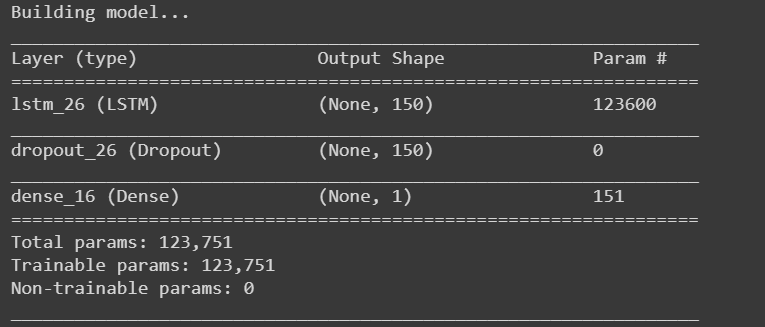
\includegraphics[width=.9\textwidth]{img/lstm_150.PNG}  
\caption{LSTM architecture with one layer}
\label{fig:lstm-150}
\end{figure}
%

we implemented an early callback to stop training before over-fitting if the loss value did not change after 2 epochs, a chart is showing the training set and test set loss during training this way we can monitor the training process.
In the figure below \ref{fig:verbose}, we can see that the test loss is lower than the training loss that is a good sign to  according to the evaluation model we saw in the previous chapter as we should always follow the bias-variace tradeoff \ref{variance_bias}.

%
\begin{figure}[h]
\centering
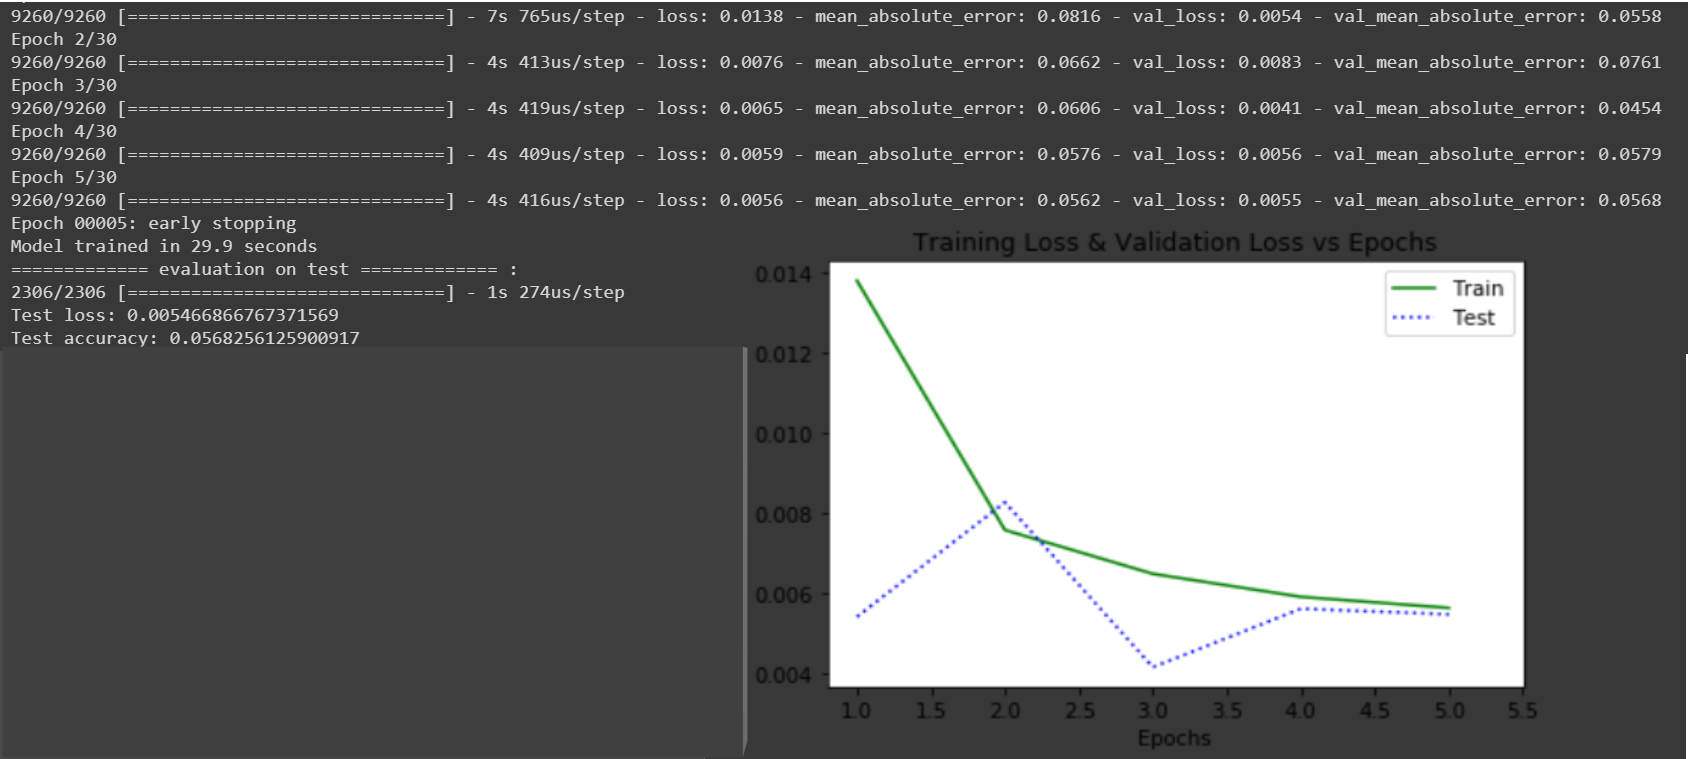
\includegraphics[scale=.4]{img/_verbose.PNG}  
\caption{cal loss}
\label{fig:verbose}
\end{figure}
%
The trained model is run on the test set which would then collect all predictions and calculate an error score. another metric was calculated for comparison; since RMSE is criticized for its over-biasing when measuring continuous variables.
\cite{Chai_Draxler_2014}.\\Next step we can visualize how well our model can predict the target training data, 
%
\begin{figure}[h]
\centering
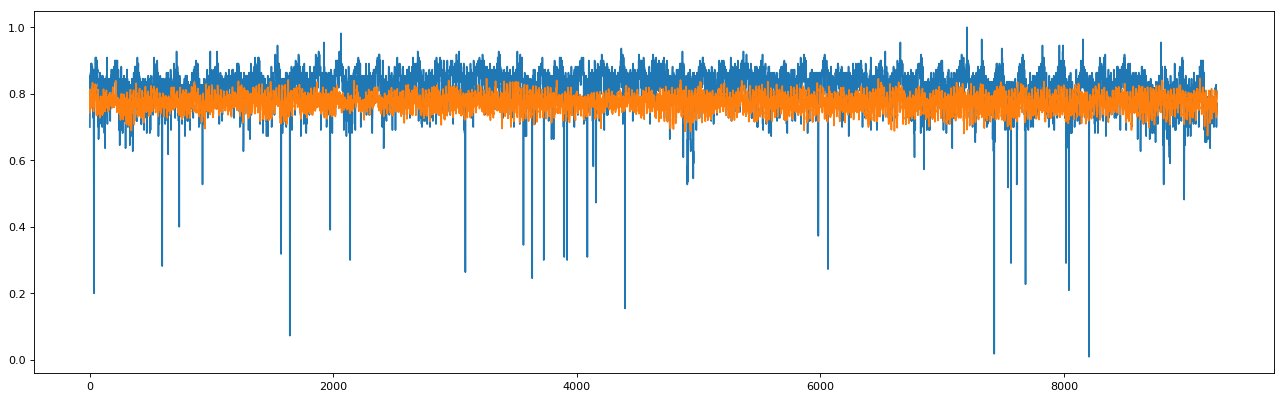
\includegraphics[scale=.4]{img/prevision_sur_training.png}  
\caption{prediction on training data set}
\label{fig:verbose}
\end{figure}
%
%
\begin{figure}[h]
\centering
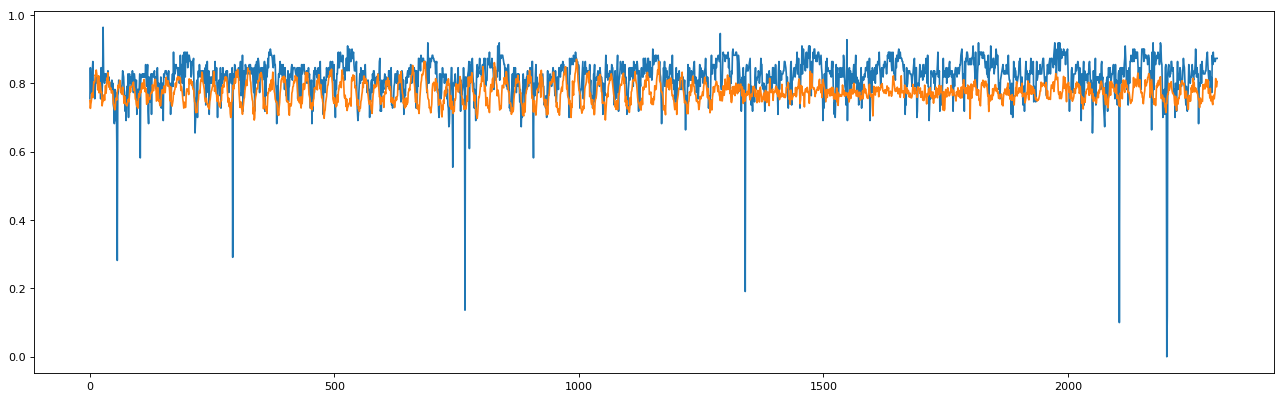
\includegraphics[scale=.4]{img/prevision_sur_test.png}  
\caption{prediction on testing  data set}
\label{fig:verbose}
\end{figure}
%
\newline
%
\begin{verbatim}
MAE : Train Score: 8.25  ,  Test Score: 7.94
RMSE : Train Score: 9.57  , Test Score: 9.62 
\end{verbatim}
%
As we can see from two figures of the prediction and the two  evaluations metrics (MAE and RMSE) we can judge that the first model with simple layer and 150 neurons, did eventually learn the seasonality and the pattern of data with an RMSE of 9.62 on testing data but still not enough to trust this model on imputing several missing hours. 

Note : one thing we should note, is that even though the MAE of training data is lower than testing data, which is normal in this case  since training data has 80\%  of original data whilst testing data is only 20\% of original data.

now we will test the model on imputation data set which has  several missing data 

\begin{figure}[h]
\centering
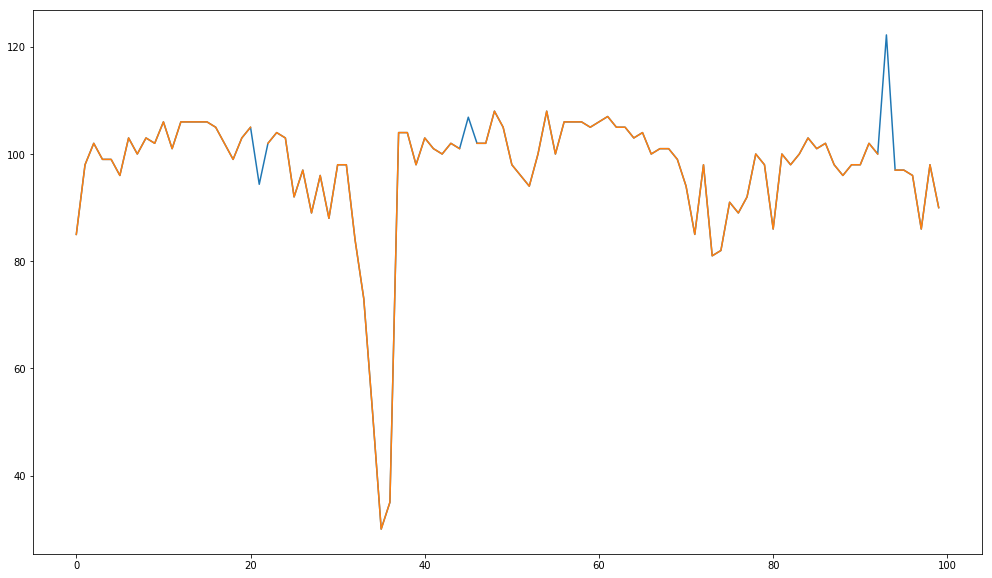
\includegraphics[scale=.32]{img/merge_best_of_result.png}  
\caption{the blue part is the imputation using  LSTM with one layer}
\label{fig:first_imp}
\end{figure}

the figure above\ref{fig:first_imp} shows the prediction of our model on the first 100 samples, and we can see that it can be in reasonable range when predicting 1h,2h. more than 3h it seems it starts to give unreasonable results, this is due to the accumulated error we have along with the prediction, in each prediction of t+1 we use the last L samples from past to impute the the future (t+1), but as in every machine learning or deep learning model the prediction always comes with an error (RMSE = 9.57). which means using the predicted values by the model to predict other future samples does have a really bad effect as we may see in the third Big gap in \ref{fig:first_imp}.

there is one way to solve this problem we suggest to increase the model complexity which will allow it to learn to generalize even better and minimize the error and for that we used another architecture  called  stateful stacked LSTM as the next figure will explain this new architecture :

\begin{figure}[h]
\centering
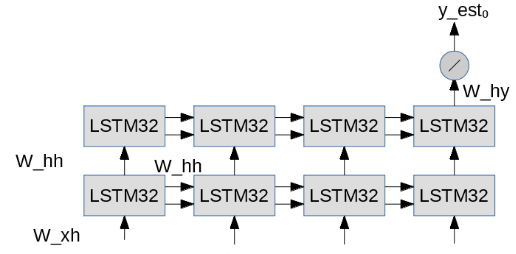
\includegraphics[width=0.55\textwidth]{img/stateful_stacked_lstm.png}  
\caption{stateful Lstm  architecture \cite{keras2015}}
\label{}
\end{figure}
we train the new model in the same data set as before and evaluate the error again using RMSE and MAE, we had the following results :
\begin{verbatim}
MAE : Train Score: 2.46  ,  Test Score: 2.09.
RMSE : Train Score: 1.94  , Test Score: 2.02 
\end{verbatim}
as we may notice that RMSE significantly dropped by using the stateful lstm architecture with different  number of neurons at each layer \ref{stat_lstm}. the training stopped at 20 epochs the val loss stopped improving.
\begin{figure}[!h]
\centering
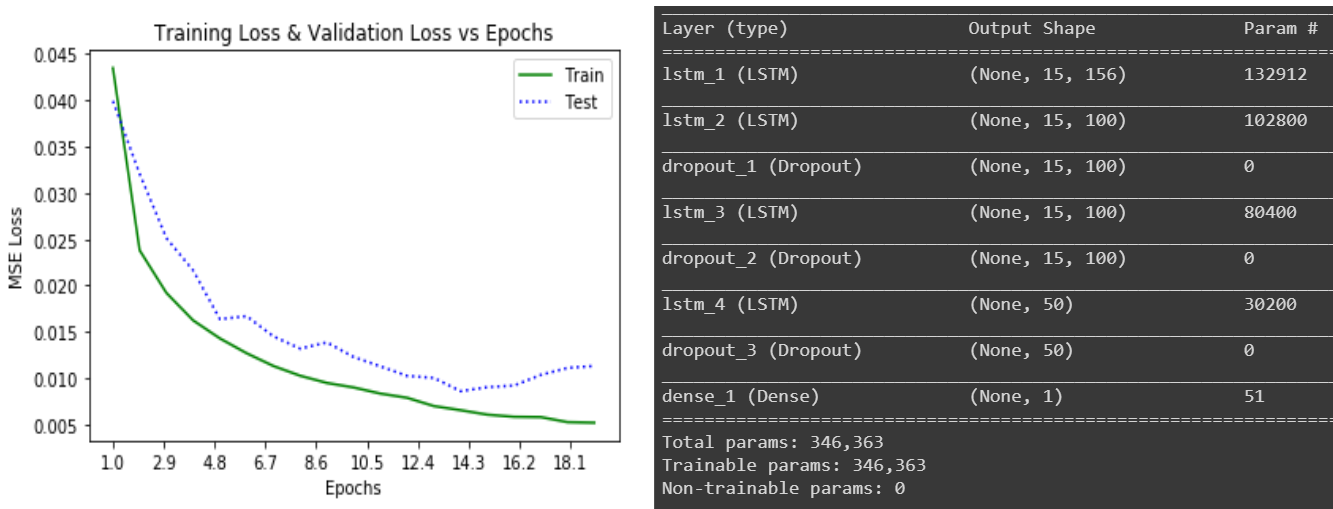
\includegraphics[width=1.06\textwidth]{img/lstm_stateful.png}  
\caption{The Stateful Lstm model and training loss vs validation Loss }
\label{stat_lstm}
\end{figure}
Now that we improved the accuracy of our model we can try and fit the model in order to estimate missing data, this time we will try it for even greater than 3h and see if it is within the possible range of the two Non missing values.
in the next figure we will visualize the first 500 of the original data that has a lot of missing data, as we can see it starts to give something really in the range.

\begin{figure}[!h]
\centering
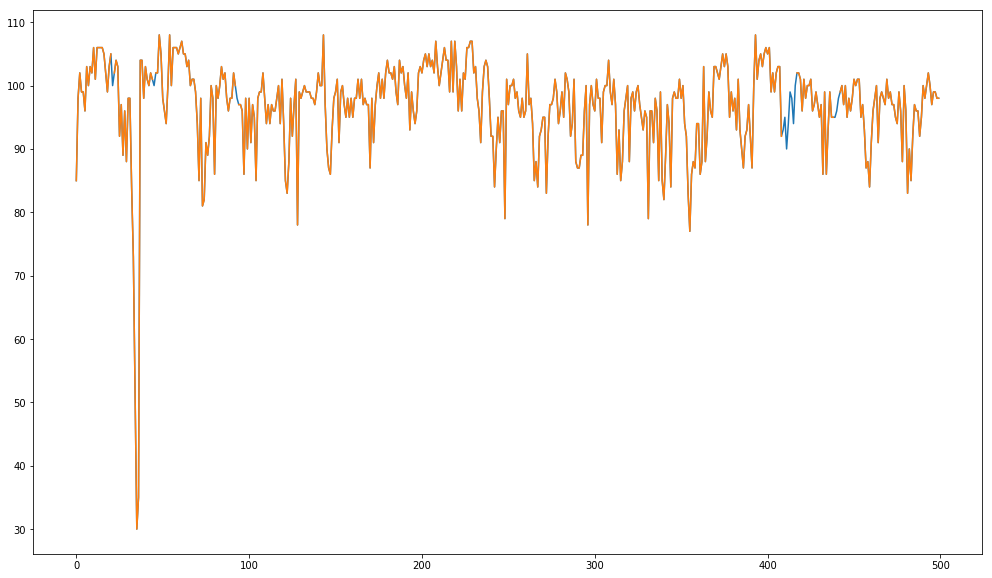
\includegraphics[scale=.4]{img/best_result.png}  
\caption{Testing the imputation}
\label{fig:verbose}
\end{figure}
the problem with our original data is that we can not quantify the error of Imputation phase, because we do not have Real values to compare our results to; in order to validate our model we would need a complete data.
we decide to  generate synthetic data, sprinkle randomly missing values or even gaps, and add features to mark the accumulated missing values, this  meta-data that indicates where the data is missing.\\the function used to  generate is $(-1)^{p}$ with $p \in N$,we trained our previous stateful model with the same parameters on 99988 samples, we let the output to be a probability, if we want perfect result we can turn the problem into binary classification with two possible outcomes -1 or +1; but we prefered to go with probability to see how it will be affected in longer gaps.
\newpage

The figure below confirms that Stateful stacked Lstm can  maintain even after 4h, with error prediction  of  0.9 in terms of RMSE, which is nearly perfect.    

\begin{figure}[!h]
\centering
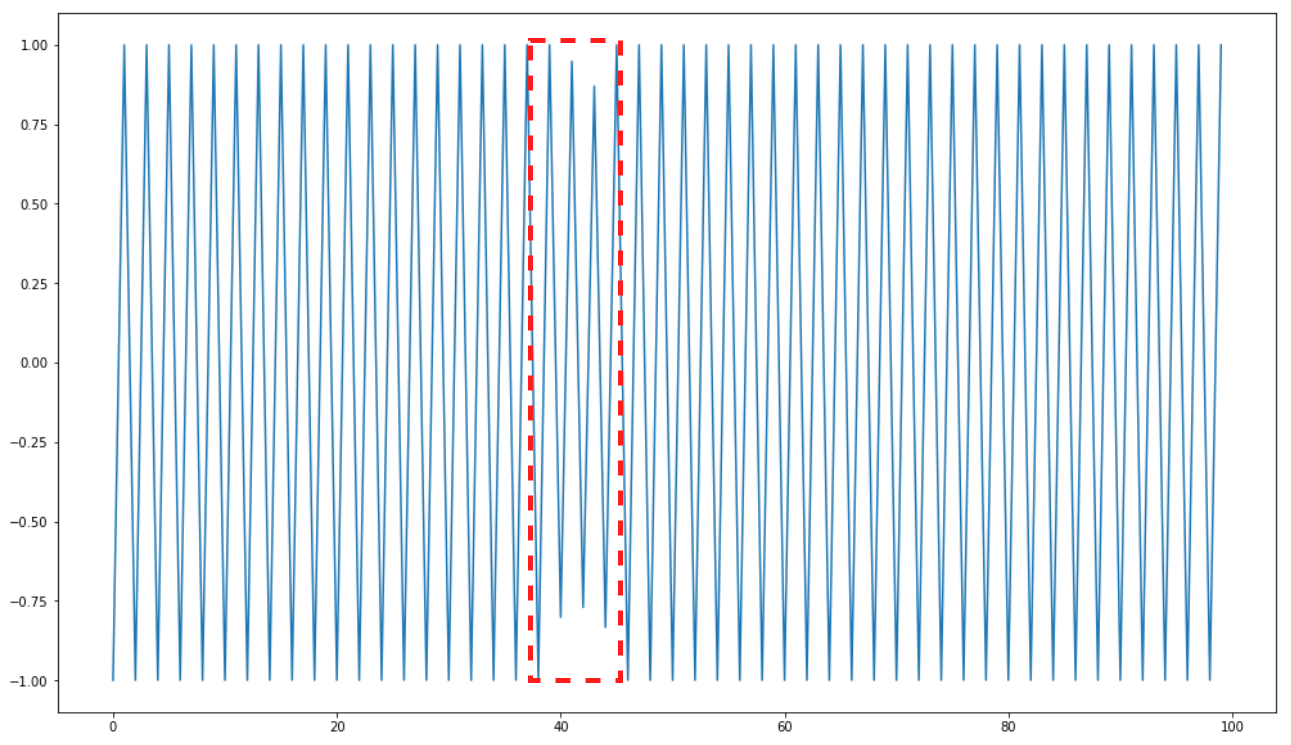
\includegraphics[scale=.4]{img/synthetic_data_lstm.png}  
\caption{Red part is the imputation of the stateful lstm }
\label{fig:state_lstm}
\end{figure}

stateful Lstm outperform all other models since it can model sequential data very good, can maintain information over time, can handle multiple variables, also can learn linear and non linear dependencies,it can  learn deep features in our data unlike ARIMA and other classical approaches.

\subsection{Time Aware LSTM (T-Lstm) }
In our experiments we tried other models as Time aware LSTM \cite{timeaware} which is a variant of  LSTM that try to inculde as input the time gaps made and based on the size of the gap we decide how  much the information flow from previous hidden states we are allowed to take in order to predict the next value ahead in the future.\\a more detailed and technical explanation of how T-Lstm work as authors  Baytas, Inci M.\cite{timeaware} explains : \say{Time Aware LSTM (T-LSTM) was designed to handle irregular elapsed times. T-LSTM is proposed to incorporate the elapsed time information into the standard LSTM architecture to be able to capture the temporal dynamics of sequential data with time irregularities. T-LSTM decomposes memory cell into short-term and long-term components, discounts the short-term memory content using a non-increasing function of the elapsed time, and then combines it with the long-term memory}.
unfortunately the T-Lstm failed to fit the training. and was not capable of learning the patterns nor imputing missing data \ref{fig:tlstm}.
\begin{figure}[H]
\centering
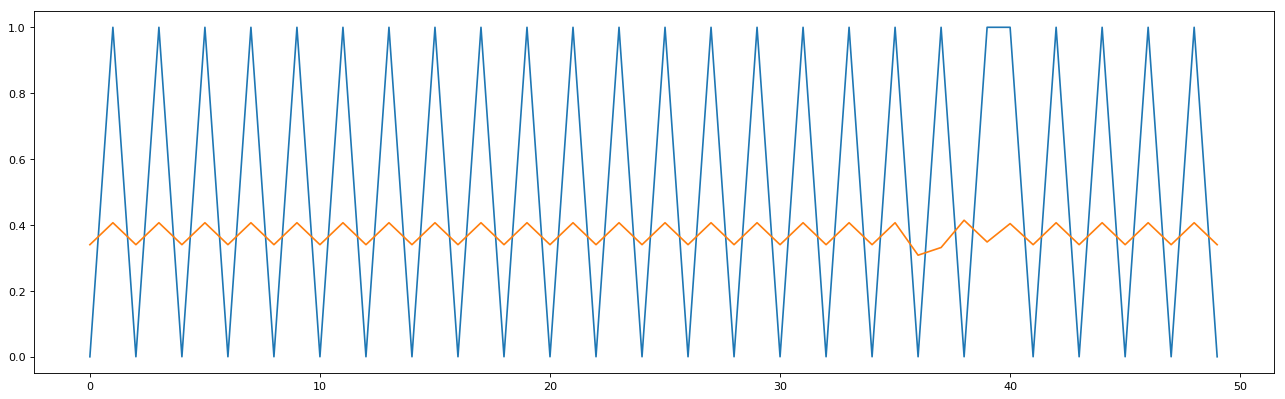
\includegraphics[scale=.4]{img/T_lstm.png}  
\caption{Time aware Lstm failing to learn the pattern of our data.}
\label{fig:tlstm}
\end{figure}

another machine learning model we used and already mentioned in state of the art chapter is Adaboost(Adaptive Boosting) can be another good option for either Forecastign time series or even imputing data the only inconvenient we have is that it needs some kind of feature extractor from our time series we used tsfresh\cite{} which provide us with 100 feature to train our model with added to our original time series with One variable (as ARIMA).
to get around the " The Curse of dimensionality " we usually use some kind of dimensionality  reduction technics as PCA, SVD or Feature engineer to reduce number of features that can make time of calculations polynomial rather than exponential.

\begin{figure}[!h]
\centering
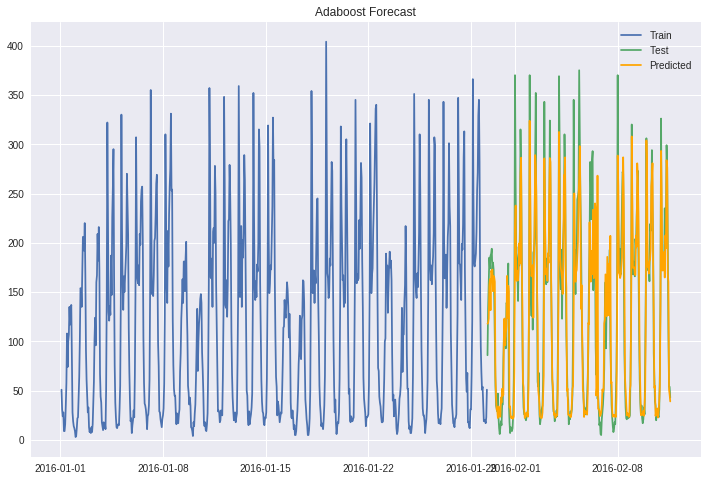
\includegraphics[scale=.6]{img/adaboost_results.png}  
\caption{Adaboost forecasting}
\label{fig:adaboost}
\end{figure}


\subsection{Transfer Learning}
Very much like one's ability to steer a car helps in learning to drive a motorcycle, the knowledge of a model contains by having been trained on one specific task might help in solving a related task.\\This is the general aim of transfer learning: to transfer knowledge from an already trained model to a different domain or a different task.\\ in our use case Transfer learning was never used before to impute missing data for a damaged sensor, it is still a low researched field. Nevertheless, to solve some issues as stated in first section of this chapter \ref{contextofimp}. our proposed solution is to use transfer learning of The nearest Neighbor of the damaged sensor that respect a number of  criterion  such as measuring the same physical property (temperature, humidity...),being at the same height, and spatially correlated. having trained LSTM for each sensor, we can easily transfer learning of one sensor into another damaged sensor in order to impute in real time. All in all, domain adaptation for IOT sensors, is a fresh idea and needs a lot of experiments on the field. However the idea is already working in a number of fields as "style transfer" for images and art \cite{transferlearning}, NLP openAI released their GPT-2 which made it possible for people to use transfer learning to customize their models, more on this subject on \cite{nlp},   



\section{Conclusion}
the reccurent neural networks are good for modeling sequential data whether it is in text data, or Time series, other variants or RNN can be tested also such as  Gated Recurrent Network, which is a variant of the LSTM. There is also the Attention Network that considered now the state of the art in NLP field, which is also a variant of LSTM. and Bidirectional LSTM means allowing information to flow not only from left to right but also of from right to left, the two sides are concatenated, and then make predictions. 

% Please add the following required packages to your document preamble:
% \usepackage{graphicx}
\begin{table}[H]
\centering
\resizebox{\textwidth}{!}{%
\begin{tabular}{c|l|l|l|}
\cline{2-4}
\multicolumn{1}{l|}{} & \multicolumn{1}{c|}{RMSE \& MAE on Trafic data} & Univariate data & Multivariate data \\ \hline
\multicolumn{1}{|c|}{\begin{tabular}[c]{@{}c@{}}Classical Approaches\\ (interpolations,mean,listwise deletion)\end{tabular}} & Not Stable almost Random & Only & No \\ \hline
\multicolumn{1}{|c|}{\textbf{ARIMA}} & \begin{tabular}[c]{@{}l@{}}MAE : Train Score: 3.48 , Test Score: 2.2\\ RMSE : Train Score: 3.53 , Test Score: 3.62\end{tabular} & Only & No \\ \hline
\multicolumn{1}{|c|}{\textbf{LSTM}} & \begin{tabular}[c]{@{}l@{}}MAE : Train Score: 8.25 , Test Score: 7.94\\ RMSE : Train Score: 9.57 , Test Score: 9.62\end{tabular} & Yes & Yes \\ \hline
\multicolumn{1}{|c|}{\textbf{Stacked LSTM}} & \begin{tabular}[c]{@{}l@{}}MAE : Train Score: 2.46 , Test Score: 2.09.\\ RMSE : Train Score: 1.94 , Test Score: 2.02\end{tabular} & Yes & Yes \\ \hline
\multicolumn{1}{|c|}{\textbf{T-LSTM}} & RMSE : Train Score: 50.8 , Test Score: 56.2 & Yes & yes \\ \hline
\end{tabular}%
}
\caption{summary comparison of some of methods we tested}
\label{tab:my-table}
\end{table}



% \section{Acknowledgments}